% This is the root file of your thesis: thesis.tex
% A line starting with % is a comment. In some cases, I have included a command preceded by a %. You may activate the command by removing the %.

%%===================================
\documentclass[12pt]{report}
\usepackage{ramsstyle}
\usepackage[final]{pdfpages}
%%===================================
%Write the various parts of your thesis as separate files and include them into the main file by the command \include{name of included file}. When you compile the LaTeX file, you may choose which subfiles to include by the command

%\includeonly{chapter01,chapter02}

%%===================================
\begin{document}
%This is the Titlepage
%%=========================================
\thispagestyle{empty}

%\mbox{}\\[3pc]
%\hrulefill
\begin{center}

\Large{NTNU}\\
\normalsize{Norwegian University of Science and Technology}\\
[3pc]
\Large{TFE4520 - SPECIALIZATION PROJECT}\\

\Huge{\hrulefill\\Sensor Data Acqusition for Ultra Low Power Applications\\\hrulefill}\\[2pc]

\small{\textit{Author:}}\\\Large{Erlend Hestnes}\\
\mbox{}\\[3pc]
\large{December 19, 2015}\\[2pc]

\small{Supervisor 1: Trond Ytterdal} \\
\small{Supervisor 2: Øystein Moldsvor}

\end{center}
\vfill

\begin{figure}[h]
\centering

\includegraphics[scale=0.5]{fig/NTNU.png}
\label{fig:frontpage_logo}
\end{figure}
 % This is the titlepage
\setcounter{page}{0}
\pagenumbering{roman}
%This is the Preface
%%=========================================
\addcontentsline{toc}{section}{Abstract}
\begin{center}
\section*{Abstract}
\end{center}

Internet of Things (IoT) applications very often involve the use of sensors. Motion sensing can be used in a vast amount of applications and are therefore very interesting in high volume IoT products. Replacing a battery in such an application is often undesirable, and may in some cases be close to impossible. It is therefore essential for such applications to have sensors that consumes as little power as possible. 

This project thesis presents a thorough analysis of five commercially available microelectromechanical (MEMS), 3-axis accelerometers. The analysis focuses primarily on finding the sensor that gives the best trade-off between functionality and power consumption, with a slightly larger emphasis on the latter. The best sensor is then chosen to be a part of a custom reference board, of which also was designed during this thesis.

The reference board is planned to be used for a Master thesis, where the goal is to further explore different IoT application areas for ultra low power motion sensors.

The project is carried out as feasibility analysis for Disruptive Technologies AS in conjunction with the Norwegian University of Science and Technology (NTNU).

\begin{center}
Trondheim, 2015-12-16\\[1pc]
\begin{figure}[h]
\centering

\includegraphics[scale=0.5]{fig/underskrift.png}
\label{fig:underskrift}
\end{figure}
Erlend Hestnes
\end{center}
%%This is the Preface
%%=========================================
\addcontentsline{toc}{section}{Preface}
\section*{Preface}

Internet of Things (IoT) applications very often involve use of sensors. Motion sensing can be used in a vast amount of applications and are therefore very interesting in high volume IoT products. Replacing a battery in such an application is often undesirable, and may even in some cases be impossible. It is therefore essential for such applications to have sensors that consumes as little power as possible. This project thesis elaborates on different techniques to acquire data from an accelerometer at the lowest possible power consumption. 

The project is carried out for a Norwegian company called Disruptive Technologies in conjunction with the Norwegian University of Science and Technology.

%Here, you give a brief introduction to your work. What it is (e.g., a Master's thesis in RAMS at NTNU as part of the study program xxx and\ldots), when it was carried out (e.g., during the autumn semester of 2021). If the project has been carried out for a company, you should mention this and also describe the cooperation with the company. You may also describe how the idea to the project was brought up.\\[2cm]

\begin{center}
Trondheim, 2015-12-16\\[1pc]
\begin{figure}[h]
\centering

\includegraphics[scale=0.5]{fig/underskrift.png}
\label{fig:underskrift}
\end{figure}
Erlend Hestnes
\end{center}
%%This is the Acknowledgment
%%=========================================
\addcontentsline{toc}{section}{Acknowledgment}
\section*{Acknowledgment}

%I would like to thank the following persons for their great help during \ldots

%If the project has been carried out in cooperation with an external partner (e.g., a company), you should acknowledge the contribution and give thanks to the involved persons.

%You should also acknowledge the contributions made by your supervisor(s).

The majority of work in this thesis has been done quite independently, without too much intervention from any of the supervisors. I would however like to thank Øystein Moldsvor for his help in steering the report in the right direction.

I would like to thank Øystein Moldsvor in helping me....

I would also like to thank Trond Ytterdal for approving the idea for this report, as well as the aid he gave me in providing useful insight on the overall report structure. 

\begin{flushright}
E.H.\\[1pc]
\end{flushright}
%%This is the Summary
%%=========================================
\addcontentsline{toc}{section}{Summary and Conclusions}
\section*{Summary and Conclusions}
%Here you give a summary of your your work and your results. This is like a management summary and should be written in a clear and easy language, without many difficult terms and without abbreviations. Everything you present here must be treated in more detail in the main report. You should not give any references to the report in the summary -- just explain what you have done and what you have found out. The Summary and Conclusions should be no more than two pages.
\tableofcontents
\setcounter{page}{0}
\pagenumbering{arabic}
%This is chapter 1
%%=========================================
\chapter{Introduction}

\section{Internet of Things (IoT)}

The IoT has a total potential economic impact of \$3.9 trillion to \$11.1 trillion a year by 2025. At the top end, that level of value—including the consumer surplus—would be equivalent to about 11 percent of the world economy \cite{mckinsey15}. Naturally, a vast amount of semiconductor companies want to be a part of this huge market, and a lot of these companies are therefore increasing their product portfolio to be ready to meet the IoT demand. 

\subsection{What Is IoT}

The Internet of Things (IoT) refers to the ever-growing network of physical objects that feature an IP address for Internet connectivity, and the communication that occurs between these objects and other Internet-enabled devices and systems \cite{webopedia}. Three very important keywords when it comes to IoT is connectivity, ease-of-use and low-power. A successful realization of the IoT movement is accelerated by creating solutions that are practical and easy to deploy ubiquitously. Low power, reliable wireless sensor networks translates into no wires and no worries for both customers and developers \cite{embedded_IoT}. 

\subsection{A Problem with IoT}

It is quite reasonable to assume that you eventually will have more than a hundred IoT devices in your home. Say that each of these devices are using a battery, and that the average battery time for each device is about one or two years. Then you would have a huge job at hand for changing the batteries as they would ultimately run out of power. For the IoT market to be successful and fully appreciated by the customers, one need to be able make devices that does not require the user ever changing the battery. This is certainly a possibility as semiconductor companies continues to push the boundaries for ultra low power components.  

\subsection{Sensors for IoT}

This project thesis focuses on a big part of IoT-applications, namely sensors. In it's broadest definition, a sensor is an object whose purpose is to detect events or changes in its environment, and then provide a corresponding output \cite{wikipedia_sensors}. They are used in vast number of applications and are considered to be a fundamental building block of the IoT. This thesis targets a specific type of sensor that is used to detect motion, specifically accelerometers. The thesis presents a thorough analysis of five commercially available microelectromechanical (MEMS) 3-axis accelerometers. The analysis focuses primarily on power consumption, but other considerations are also taken into account. Based on this analysis, an accelerometer is chosen to be used in a demo application.

\subsection{Thesis Outline}

[The motivation behind this thesis is to show some of the potential IoT applications that can be achieved by using low-power features, found on modern microcontrollers, to acquire data from an ultra-low power accelerometer.]

\textbf{Chapter 2 - Background Theory:} This section presents relevant background theory regarding accelerometers, microelectromechanical systems (MEMS) and common low-power techniques.  

\textbf{Chapter 3 - Accelerometer Overview:} An extensive description of five ultra low power, commercially available MEMS accelerometers

\textbf{Chapter 4 - Accelerometer Analysis:} Presents an analysis around choosing one of the accelerometers from Chapter 3 for a demo application.

\textbf{Chapter 5 - Demo Application:} This chapter presents the demo application.

\textbf{Chapter 6 - Possible IoT Applications:} Discusses some potential IoT application

\textbf{Chapter 7 - Results:} Presents the results from power measurements on the demo board

\textbf{Chapter 8 - Conclusion:} Concludes the work in the report.


\chapter{Background Theory}
\label{chap:theory}

To understand the rest of this thesis, some basic knowledge about low power design, accelerometers in general and microelectromechanical systems (MEMS) are required. This chapter presents an overview of these topics. The theory presented in this chapter should be regarded as well-established, and is covered in several books and papers.

It is assumed that the reader has a good understanding of embedded systems, as well as some knowledge of basic physical principles. 

\section{Low power design}

A successful realization of the IoT requires devices that can operate their entire lifespan on a very small battery. A battery is basically an energy container, and for non-rechargeable batteries this energy is a limited resource. Power is the rate at which energy is consumed, which means that reducing the power consumption translates into longer battery life \cite[~p.3]{holberg06}. The following section presents the two main contributors to power consumption in a modern CMOS circuit. 

\subsection{Power in CMOS}
\label{sec:cmos_power}

The power consumption in CMOS circuitry can in general be divided into two different domains, static and dynamic power consumption. Static power consumption ($P_{static}$) comes from leakage current in the transistor, which is a result of reverse-bias leakage between diffused regions and the
substrate in the transistor \cite{static_dynamic_power}. The static power consumption is given by the product of the static current ($I_{static}$) and the supply voltage ($V_{ss}$), as seen in Equation \ref{eq:p_static}. 

\begin{equation}
P_{static} = I_{static} \cdot V_{ss}
\label{eq:p_static}
\end{equation}

Dynamic power consumption ($P_{dynamic}$) is result of switching the logic state of the transistor, which is given by the sum of the transient- and capacitive load power consumption. The transient power ($P_{transient}$) consumption is from the current that flows through the transistor when the the transistor is switching logic state, while the capacitive load power ($P_{capacitive}$) is from the additional current consumed in charging external load capacitance ($C_{L}$) \cite{cmos_power_consumption}. The dynamic power consumption is dependent on the frequency ($f$) as well as the number of transistors that are switching ($N$). The dynamic power consumption is also proportional to the supply voltage ($V_{ss}$) squared. This relationship can be seen in Equation \ref{eq:p_dynamic}.

\begin{equation}
P_{dynamic} = P_{transient} + P_{capacitive} = (C_L + C) \cdot V_{ss}^{2} \cdot f \cdot N^3
\label{eq:p_dynamic}
\end{equation}

From Equation \ref{eq:p_dynamic} one can see that the dynamic power consumption is proportional to the frequency. This means that a higher performance generally leads to a higher power consumption. Another important aspect to note, is that the supply voltage is present both in the static and dynamic power consumption of CMOS circuits. Reducing the voltage is therefore very important when it comes to reducing the overall power consumption in a CMOS circuit.

\subsection{Power saving peripherals}

Information is always represented as states of variables in a physical system. Energy is consumed when changing or preserving such a state. In order to save energy, one therefore needs reduce the amount of information being processed. Which further implies that in order to save power, one needs to reduce the rate of information processing \cite{sarpeshkar12}.

Modern microcontrollers feature several advanced peripherals which can be utilized to do certain operations more efficient, thereby saving power. In the following sections we are going to look at some of these peripherals.

\subsubsection{DMAC - Direct memory access controller}

A Direct Memory Access Controller (DMAC) is basically a peripheral device that can be configured to move data from one location in memory to another. Since peripheral devices almost always are memory mapped in a microcontroller, a DMAC is usually also able to transfer data from and to peripherals as well. 

Direct Memory Access is primarily used as a technique to offload the CPU for large data transfers, as these operations can be very time consuming for the CPU to perform. It is also more power efficient to use a DMAC for such data transfers, since the DMAC both consumes less power and transfers data more efficient than the CPU. The DMAC is also able to work independently of the CPU, which means that the CPU can either do other work or sleep while the the DMAC is moving data. The former can be used to increase the overall system performance, while the latter can be exploited to achieve greater power efficiency \cite{ball03}.

\subsubsection{Event system}

An event system enables different peripherals in the microcontroller to interact autonomously with each other by using tasks and events. By using such a system one is able to let peripherals communicate with each other without involving the CPU. This can be exploited to do certain operations while the CPU is sleeping, thereby saving power.

\subsubsection{Clock gating}

A clock gating scheme is all about turning off the clock for the unused domains of the chip. Clock gating effectively removes the dynamic power consumption from the gated domain, which can be seen from Equation \ref{eq:p_dynamic}. The static power consumption is however still present, as voltage is still applied to the gated domain. Clock gating can for example be beneficial for volatile memory (such as SRAM), as the user can reduce power consumption while still maintaining data in memory \cite{gupta14}.

\subsubsection{Power gating}

Power gating is about completely turning off the voltage to unused blocks of the system, thereby removing both static and dynamic power consumption. Modern microcontrollers often have the ability to power gate SRAM blocks, giving the user the option to trade power for RAM \cite[p.~24]{nrf51}. It is also common to power gate peripherals that are not used for the application.

\subsubsection{Power modes}

Both clock gating and power gating are usually incorporated into different power modes. Some of these modes may offer a complete shutdown of the entire circuit, while others enables the user to shut down sections or peripherals that are not in use. The advantage of having multiple power modes is the flexibility it provides to shut down any part of the microcontroller that is not absolutely necessary to function at hand \cite[~p.4]{holberg06}.  

%\subsection{Energy Harvesting}

%[still don't know where to put this section]

%A battery will always run out of power, no matter how little current the system draws. So to be able to make a system that can continue indefinitely, one need to be able to have an infinite power source. Unfortunately, this does not exist. There is however a lot of research going into developing solutions that can turn energy from our surroundings into electrical energy. The principal is called energy harvesting, and it is truly a term that goes hand in hand with the IoT movement. Energy can be harvested from vibrations, sunlight, heat and a lot of other sources. A product that can implement one or more of these energy harvesting techniques has the potential to run indefinitely. Energy harvesting is something that has existed for a long time, but it is only with today's ultra low power components that it is actually possible to use this energy to power our devices.

\section{Accelerometers - Working principle} \label{sec:accel_working_principle}

Acceleration is defined as the rate of change in velocity with respect to time. It is given by a vector with both magnitude and direction relative to a reference frame. The SI units are length divided by time squared \cite{elert98}.

The working principle of an accelerometer can be viewed as a simple mechanical system, as illustrated in Figure \ref{fig:accel_working_principle}. A proof mass $m$ is connected to a frame by a flexible spring $k$. When an acceleration is imposed along the x-axis, the proof mass will begin to move. Due to Newton's law of inertia, the motion of the proof mass will lag the frame motion \cite[~p.34]{kaajakari09}. This will cause an oscillation of the proof mass inside the frame. From this oscillation alone, it is possible to get the acceleration. However, to prevent excessive oscillation, the mass vibrations are usually damped by introducing a dampening material (such as gas or liquid) inside the package. This is represented by a dashpot $\gamma$ in Figure \ref{fig:accel_working_principle}.

\begin{figure}[h]
\centering
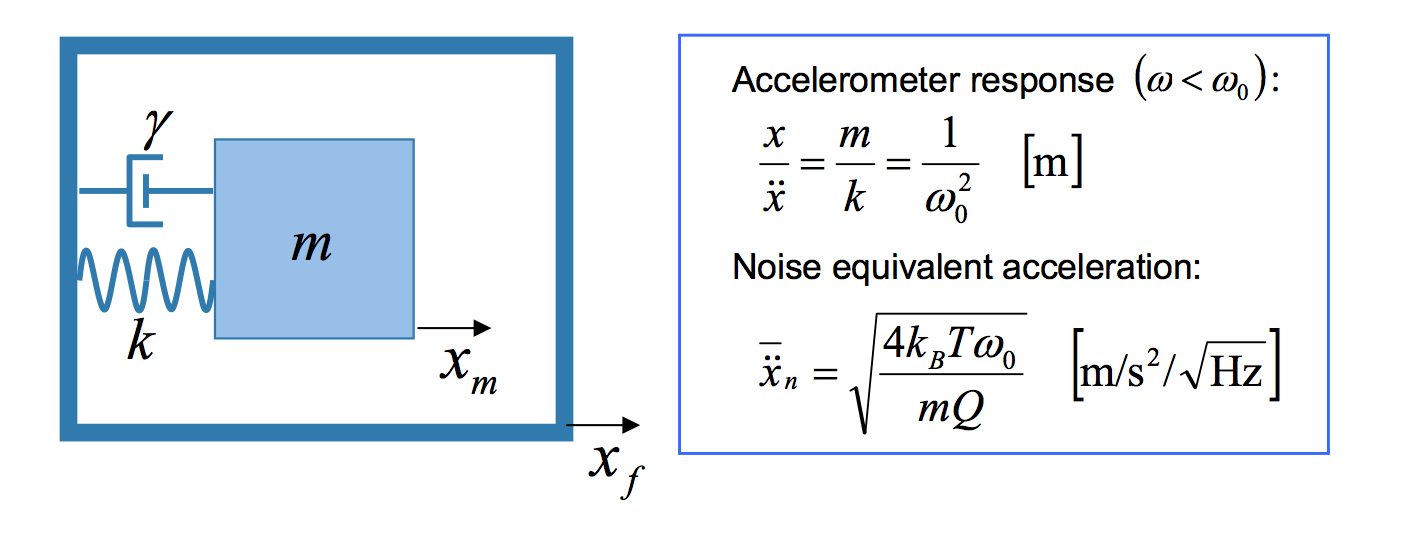
\includegraphics[scale=0.5]{fig/accelerometer_working_principle.png}
\caption{Working principle of an accelerometer \cite[~p.34]{kaajakari09}}
\label{fig:accel_working_principle}
\end{figure}

\subsubsection{Mechanical noise in accelerometers}
\label{sec:mechanical_noise}
The mechanical noise in an accelerometer is usually specified by the power spectral density (PSD), given by Equation \ref{eq:noise_spectral_density}. If we analyse this equation more closely, we see that the thermal noise energy $k_b T$ is a constant irrespective of the system size \cite[~p.13]{kaajakari09}. This means that the thermal noise induced in mechanical vibrations sets the lower limit for the smallest, measurable acceleration \cite[~p.41]{kaajakari09}. One can also see from Equation \ref{eq:noise_spectral_density} that increasing the mass $m$ and reducing the resonant frequency $\omega_0$ reduces the overall noise. The $Q$ factor, or quality factor, is a dimensionless parameter that describes how under-damped an oscillator or resonator is \cite[~p.216]{harlow04}. Again, we can see from Equation \ref{eq:noise_spectral_density} that increasing the Q factor helps reducing the overall noise.

\begin{equation}
\bar{\ddot{X_{n}}} = \sqrt{\frac{4 k_b T \omega_0}{mQ}}
\label{eq:noise_spectral_density}
\end{equation}

\section{Microelectromechanical systems (MEMS)}

Microelectromechanical Systems (MEMS) are embedded systems involving one or many micromachined components or structures \cite[p.~3]{maluf04}. The technique is used for a vast number of applications ranging from accelerometers and gyroscopes to fluid nozzles on an inkjet printer.

\subsection{MEMS accelerometers}

The basic working principles of an accelerometer, described in section \ref{sec:accel_working_principle}, also applies for all types of MEMS accelerometers. The different MEMS accelerometers do however differ in the way that they sense the displacement of the inertial mass. One of the most common methods involve sensing the change in capacitance when the inertial mass is displaced, then converting it into an amplified output voltage. Another method involves sensing the internal stress in the spring by using piezoresistors. One also see solutions were the spring is replaced with a piezoelectric element, providing a voltage in direct proportion to the displacement itself.

The first micromachined accelerometer was demonstrated at Stanford University in 1979. However, it took nearly 15 years for the technology to become accepted into mainstream products \cite[p.~8]{maluf04}. The automotive industry has undoubtedly been a big contributor for the technology, as accelerometers has an apparent application in detecting crashes for airbag deployment systems. MEMS accelerometers has in recent years also found its way into other applications, such as smart phones, quad-copters and game controllers \cite{digikey_mems_guide_2}. 

\subsection{MEMS processing techniques}

The following sections presents the most common processing techniques for MEMS elements.  

\subsubsection{Surface micromachining}

Surface micromachining is based on patterning deposited thin film materials on top of a substrate wafer \cite[p.~5]{kaajakari09}. The production technique first appeared in the 1980s, and was primarily used as a low cost alternative to accelerometers for the automotive industry \cite[p.~101]{maluf04}. However, recent improvements in the production technique has made it possible to use the technique for other sensors such as pressure sensors, gyroscopes and microphones. 

The surface micromachining process bear a close resemblance to the traditional integrated circuit (IC) manufacturing process, which is also based on processing thin films on a silicon wafer. In fact, the processes are so close that a retired IC manufacturing plant often are converted into a MEMS fabrication plant, as MEMS does not require the latest in fabrication technology \cite[p.~4]{kaajakari09}. The similarities between IC manufacturing and surface micromachined MEMS has several advantages. It is for instance relatively easy to integrate MEMS architectures together with IC to make a single-chip solution, which often leads to better performance and reduced packing-cost \cite{mcube_fact_sheet}. 

\subsubsection{Surface micromachined accelerometers}

Surface micromachined accelerometers incorporates a comb-like structure, as depicted in Figure \ref{fig:surface_micromachined}. The primary axis is located in the plane of the die, and is often referred to as an x-axis or y-axis. Two sets of electrodes are anchored down in the substrate. These two electrodes are interlaced with a third set connected to the inertial mass. This mass is being suspended over the surface by means of two long beams, acting as a suspension spring. Thereby, it is free to move about as acceleration is applied along the primary axis. When the inertial mass is displaced due to an acceleration, it is causing the capacitance to change between the fingers of the comb-like structure. The change in capacitance is typically very small, in the order of 100 $\si{\femto\farad}$ \cite[p.~101]{maluf04}. To mitigate this problem, several sensing fingers are often combined in parallel to increase the overall capacitance.

\begin{figure}[h]
\centering
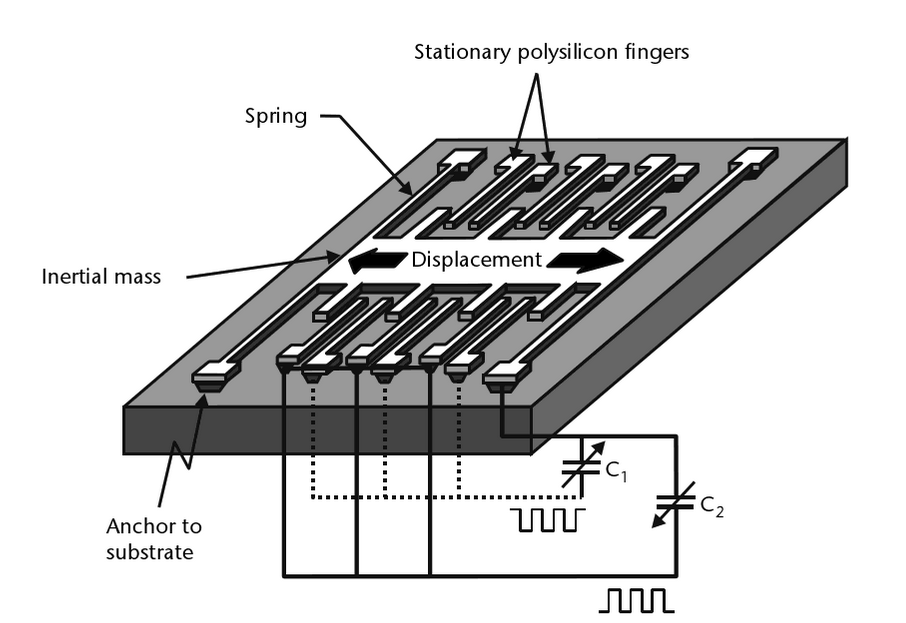
\includegraphics[scale=0.3]{fig/surface_micromachined.png}
\caption{Illustration of surface micromachined accelerometer from Analog Devices ADXL family \cite[p.~101]{maluf04}}.
\label{fig:surface_micromachined}
\end{figure}

\subsubsection{Bulk micromachining}

Bulk micromachining defines structures by selectively etching. This makes it possible to etch much thicker structures when being compared to the surface micromachining process. A typical thickness of bulk micromachined structure is between 500$\si{\micro\meter}$-700$\si{\micro\meter}$, which is about a 100 times the typical thickness of a surface micromachined structure \cite[p.~7]{kaajakari09}. A thicker structure means more mass, which is very beneficial in terms of reducing the noise, which can be seen from Equation \ref{eq:noise_spectral_density}. Bulk micromachined structures can also be made of a single-crystal silicon as opposed to thin film materials in surface micromachined structures. This is very beneficial, since these materials are very predictable and stable. Bulk micromachined accelerometers either use piezoresistive elements or capacative sensing to detect the displacement of the inertial mass \cite[p.~7]{kaajakari09}.

Pressure sensors and accelerometers were the first commercial products that utilized the bulk micromachining technique. These devices have been very successful, as 90\% of all sold pressure sensors utilize this technique. The production process is however more complicated and expensive than surface micromachining, and has therefore lost market shares in the recent years \cite[p.~7]{kaajakari09}.

\subsubsection{Piezoresistive bulk micromachined accelerometers}

Electrical resistance changes due to mechanical stress. This effect occurs in all materials and it is called the piezoresistive effect \cite[p.~73]{kaajakari09}. For an accelerometer of this type, piezoresistive springs are used to sense the displacement of the inertial mass. In general, the sensing technique offers two advantages. The resistance measurement circuitry is very simple to implement compared to that of capacitive sensors. The second is that piezoresistors are inherently shielded structures, so no hermetic packaging is required. However, piezoresistive sensing suffers from noise, as the elements themselves has a large temperature dependency, and they also consumes a significant amount of power. Because of this, sensors with this sensing technique has lost market share to capacitive sensors.

\begin{figure}[h]
\centering
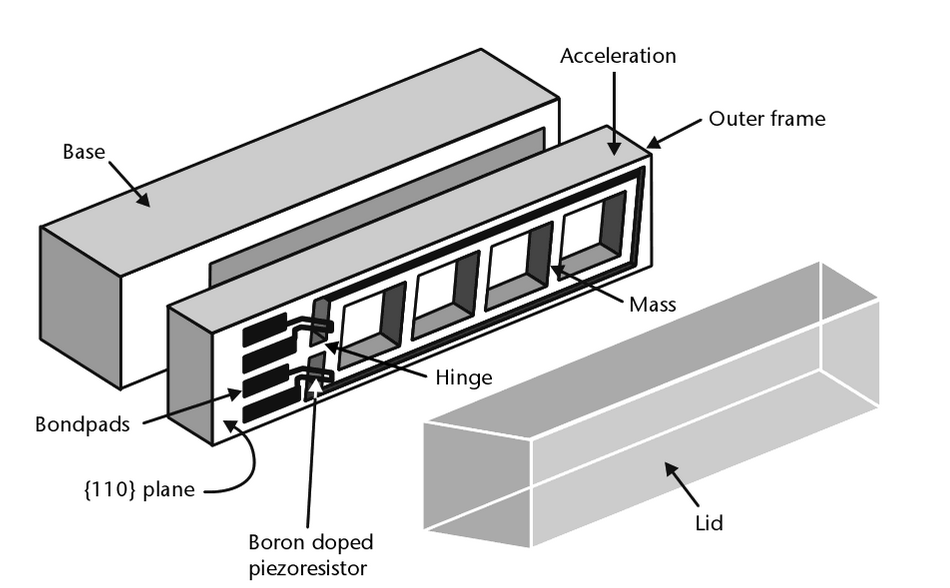
\includegraphics[scale=0.3]{fig/piezoresistive.png}
\caption{Illustration of piezoresistive accelerometer from Endevco Corp. \cite[p.~98]{maluf04}}
\label{fig:piezoresistive_accel}
\end{figure}

\subsubsection{Capacitive bulk micromachined accelerometers}

A capacitive bulk micromachined accelerometer measures the differential change in capacitance when the inertial mass is displaced. Capacitive sensors provides an excellent noise performance and low power consumption \cite[p.~91]{kaajakari09}. One of the main challenges with capacitive sensors is to accurately measure the change in capacitance, as these changes themselves are extremely small. 

\begin{figure}[h]
\centering
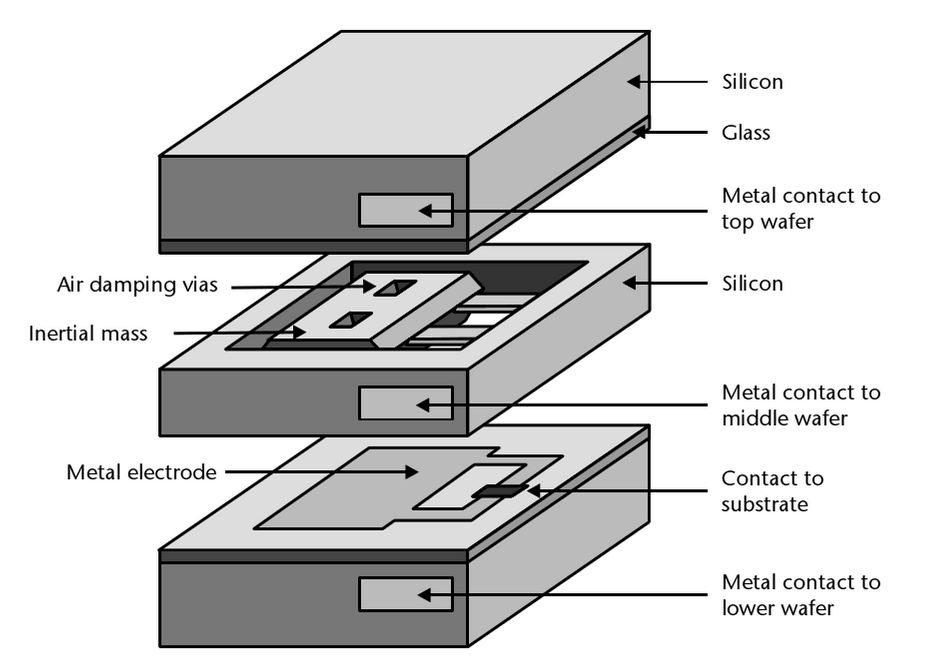
\includegraphics[scale=0.25]{fig/bulk_micromachined.png}
\caption{Illustration of capacative bulk micromachined accelerometer. \cite[p.~100]{maluf04}}
\label{fig:bulk_micromachined}
\end{figure}

\subsection{Integrating MEMS and IC's}

Most MEMS based sensors must be bonded together with an IC for integration in larger electronic systems. The MEMS element itself is just a transducer, converting some physical parameter (i.e. motion, sound, pressure) into an electrical signal. Data converters, amplifiers and signal conditioning is required to be able to make use of the signal from the transducer, which requires additional logic on an IC. A typical functional block diagram of a MEMS accelerometer can be viewed in Figure \ref{fig:ADXL362_functional}. 

\begin{figure}[h]
\centering
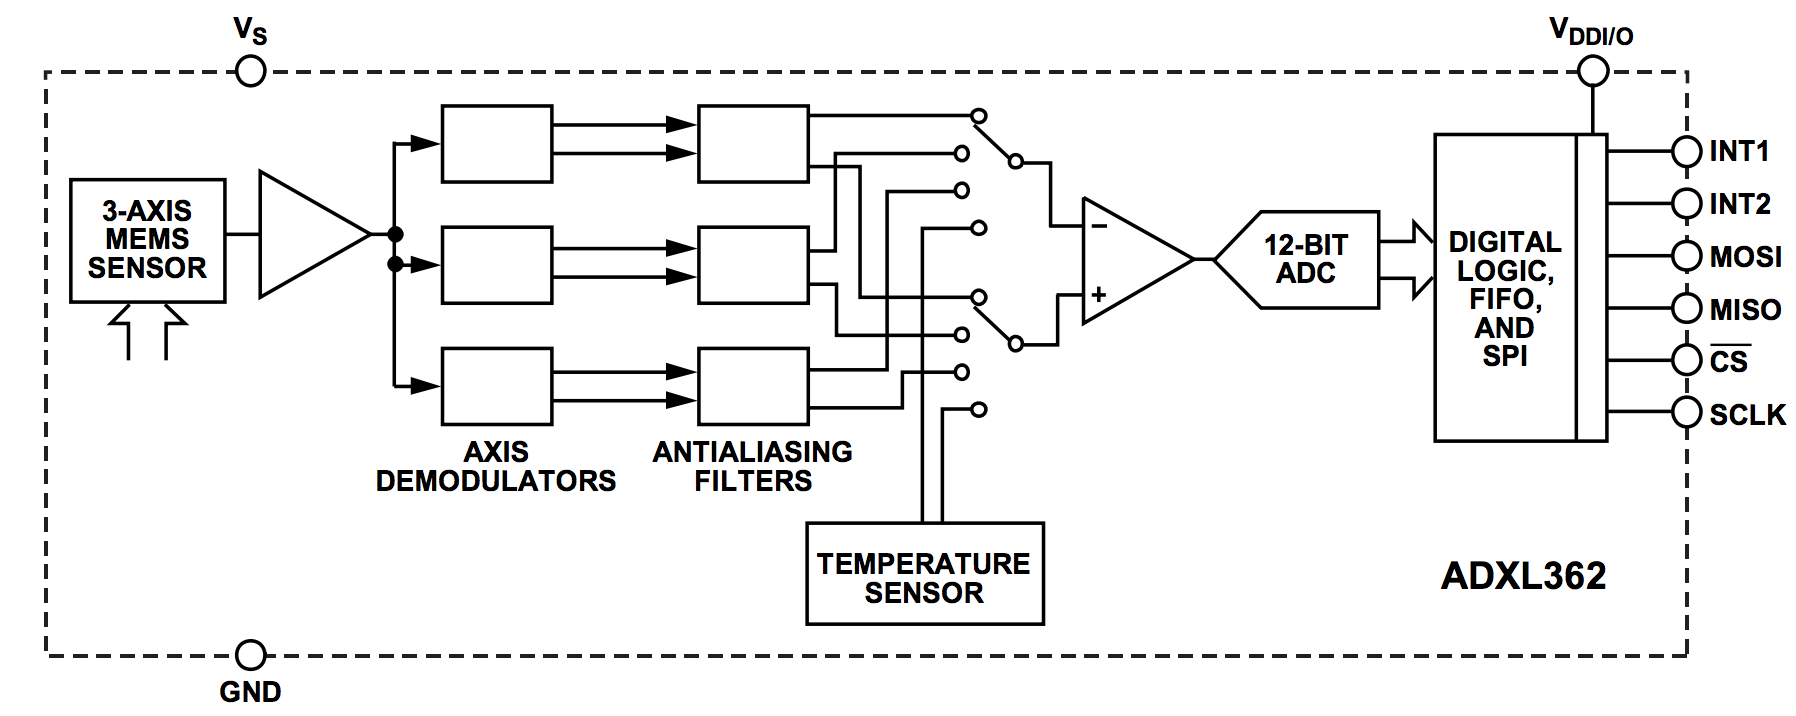
\includegraphics[scale=0.5]{fig/ADXL362_functional_block.png}
\caption{Functional block diagram of ADXL362 from Analog Devices.}
\label{fig:ADXL362_functional}
\end{figure}

MEMS and IC's can be integrated together in two separate fashions. The most common approach is to manufacture MEMS and IC's on separate substrates using their dedicated production processes respectively, and then bond them together in the final system. This approach is typically referred to as a multi-chip solution or a system-in-package (SiP), depending on whether the chips are stacked horizontally or vertically. In the other integration approach, MEMS and IC's are manufactured on the same substrate, using consecutive or interlaced processing schemes. This approach is often referred to a system-on-chip (SoC) solution \cite{fischer15}. 

\subsection{MEMS accelerometer parameters}

This section gives an overview, as well as an explanation, of the most common characteristics one should look for when selecting a MEMS accelerometer for an embedded application.

\subsubsection{Accelerometer interface}

Primarily one differentiates between two interface types when it comes to accelerometers, analog and digital. Analog accelerometers have an output that is a continuous voltage proportional to the acceleration. An analog accelerometer is therefore best suited for a completely analog circuit. An analog to digital converter (ADC) is a required peripheral for a microcontroller to make use of such a sensor in a digital system.

Digital accelerometers typically use a serial communication interface like SPI or I2C for data transfer. They are therefore much better suited for a digital circuit, as most of today's microcontrollers usually features one or both of these serial interfaces.

From a power perspective, it is worth noting that SPI is a more efficient communication interface than I2C. This is because SPI is full-duplex and generally operates at a higher clock frequency than I2C, which means that more data can be transmitted in less time \cite[p.~23]{spi}. 

\subsubsection{Number of axes}
MEMS accelerometers are able to measure acceleration along either one, two or three axes (x,y and z). Two axes (x and y) are usually sufficient for most applications, and are therefore the most common type. 3-axis accelerometers are however becoming more and more popular. Mainly because three axes are very useful for applications such as quad-copters, smart phones and game controllers \cite{digikey_mems_guide_2}.

\subsubsection{Measurement range}
Measurement range, sometimes called swing level, is defined as the level of acceleration that is supported by the sensor’s output signal specifications \cite{analog_accel_guide}. This level is listed as a number $n$ times the earth’s gravity (i.e. $\pm$1g , $\pm$2g etc.). This number is an upper limit for the accurate measurement range of the part. For example, if the part is rated with a measurement range of $\pm$3g, it means that the part can measure the acceleration accurately up to an acceleration of $\pm$3g.  If the part is accelerated above this limit, the output might rail or be distorted at the output.

\subsubsection{Sensitivity}
The sensitivity is defined as the sensor's ratio of change in mechanical input to change in electrical output. Ideally, the ratio between the acceleration and the sensor output should be linear. In practice, all MEMS accelerometers suffers from non-linearity due to mechanical stresses and circuit temperature coefficients  \cite{analog_accel_guide}. For digital accelerometers, the sensitivity is usually specified at a specific voltage as units of mg/LSB. For example, if an accelerometer has a rating of 1mg/LSB, it means that when the lowest order bit in the output changes, the acceleration has changed by 0.001 g's (1mg).

\subsubsection{Bandwidth}

The output data rate (ODR) defines the data sample rate for digital accelerometers. The bandwidth (BW) is defined as the highest frequency signal that can be sampled without any aliasing by the specified ODR. As specified by the Nyquist criterion, the bandwidth is half the output data rate \cite{analog_accel_guide}, as seen in Equation \ref{eq:bw}. 

\begin{equation}
BW = \frac{ODR}{2}
\label{eq:bw}
\end{equation}

\subsubsection{Noise}

The noise in a MEMS accelerometer is either from mechanical noise in the MEMS element, as described in Section \ref{sec:mechanical_noise}, or as electronic noise in the IC itself. The overall noise in the system is usually given by the power spectral density (PSD) in the accelerometer datasheet, usually in the units of $\si{\micro}$g per square root Hz. The PSD captures the frequency content of a stochastic process (noise) and describes how the power is distributed across different frequencies. The noise in an accelerometer is predominantly considered to be Gaussian white noise, and is thereby a constant value across all frequencies \cite{freescale_accel_guide}. The relationship between the PSD and the root-mean-square (RMS) noise is given by Equation \ref{eq:rms_noise}, and can be simplified to \ref{eq:rms_psd_bw}.

\begin{equation}
N^{2}_{rms}=\int_0^{BW}{PSD(f)df}
\label{eq:rms_noise}
\end{equation}

\begin{equation}
N_{rms}=\sqrt{PSD \cdot BW}
\label{eq:rms_psd_bw}
\end{equation}

The PSD noise value that is listed in the component datasheets is usually listed as the square root PSD from the derivation in Equation \ref{eq:rms_psd_bw}, which in turn gives us Equation \ref{eq:rms_psd_bw_2}.

\begin{equation}
N_{rms}=PSD_{datasheet} \cdot \sqrt{BW}
\label{eq:rms_psd_bw_2}
\end{equation}

\subsubsection{Digital resolution}

An accelerometers digital resolution is normally specified as the number of bits in the ADC. The devices that are available today typically range between 12 and 16-bits. However, this number might sometimes be misleading. Every MEMS accelerometer suffers from system noise to a certain extent, which in turn will limit the number of effective bits in the ADC \cite[~p.3]{freescale_accel_terminology}. In other words, it does not help to have a 16-bit ADC if four of the lower bits are full of noise. The number of effective bits (ENOB) is possible to calculate if the system noise is specified in the datasheet. One first need to calculate the system noise for a specific measurement range and bandwidth. This can be done by using Equation \ref{eq:system_noise} together with Equation \ref{eq:rms_psd_bw_2}. A measurement range of $\pm$2g (4g in total) is assumed in Equation \ref{eq:system_noise}. By combining Equation \ref{eq:effective_bits} with Equation \ref{eq:system_noise} one is able to calculate the number of effective bits. 

\begin{equation}
SNR(dB) = 20\log{\frac{\frac{4g}{2\sqrt{2}}}{N_{rms}}}
\label{eq:system_noise}
\end{equation}

\begin{equation}
ENOB = \frac{SNR(dB)-1.76}{6.02}
\label{eq:effective_bits}
\end{equation}
\chapter{Accelerometer Overview}
\label{chap:overview}

This chapter presents an overview of five of the most low power, consumer grade, MEMS accelerometers that are currently available on the market.

\section{Comparison of Ultra-Low Power Accelerometers}

Five accelerometers from five different semiconductor vendors are presented in Table \ref{tab:accel_comparison}. The accelerometers have been selected after carefully looking through the product portfolio of every semiconductor company that provides consumer grade MEMS accelerometers. The search has been constrained by only looking at accelerometers with a shutdown current of less than 1$\si{\micro\ampere}$ and a sampling current of less than 500$\si{\nano\ampere}$/Hz. The search was further constrained by only looking at 3-axis devices (X, Y and Z) with a digital interface of either SPI or I2C.

The specifications presented in Table \ref{tab:accel_comparison} are gathered from the datasheets of each individual component. All of numbers presented in Table \ref{tab:accel_comparison} denotes typical values, unless stated otherwise. The effective number of bits has been calculated for every accelerometer, by using Equation \ref{eq:effective_bits}.

\begin{figure}[h]
\begin{center}
    \resizebox{\textwidth}{!} {
    \begin{tabular}{ | l | l | l | l | l | l |}
    \hline
    \textbf{Device} & \textbf{ADXL362} & \textbf{MMA8491Q} & \textbf{MC3610} & \textbf{LIS3DH} & \textbf{KX123} \\ \hline
    
    \textbf{Manufacturer} & Analog Devices & Freescale Semiconductor & mCube & STMicroelectronics & Kionix \\ \hline
    
    \textbf{Supply Voltage} & 1.6-3.5V  & 1.95-3.6V & 1.6-3.6V & 1.71-3.6V & 1.71-3.6V \\ \hline
    
    \textbf{Shutdown current} & 10$\si{\nano\ampere}$ ,$V_s = 2.0 V$ & 1.8$\si{\nano\ampere}$ ,$V_s = 2.8 V$ & 400$\si{\nano\ampere}$ ,$V_s = 1.8 V$ & 500$\si{\nano\ampere}$ ,$V_s = 2.5 V$ & 900$\si{\nano\ampere}$ ,$V_s = 2.5 V$ \\ \hline
    
    \textbf{Max ODR} & 400Hz & 800Hz & 400Hz & 1.25/5kHz \footnote[3] & 25.6kHz \\ \hline
    
    \textbf{ODR current} & 1.8$\si{\micro\ampere}$ / 13$\si{\micro\ampere}$ \footnote[2] & 20$\si{\micro\ampere}$ \footnote[1] & 4.7$\si{\micro\ampere}$ / 14$\si{\micro\ampere}$, (FIFO On) \footnote[4] & 20$\si{\micro\ampere}$ / 10$\si{\micro\ampere}$ \footnote[3] & 21$\si{\micro\ampere}$ \\
    
    & $V_s = 2.0 V$, 100Hz ODR & $V_s = 2.8 V$, 100Hz ODR & 3.2$\si{\micro\ampere}$ / 8.4$\si{\micro\ampere}$, (FIFO Off) \footnote[4] & $V_s = 2.5 V$, 100Hz ODR  & $V_s = 2.5 V$, 100Hz ODR \\
    
    & & & $V_s = 1.8 V$, 50Hz ODR & &  \\ \hline
    
    \textbf{Sensitivity} & 1mg/LSB (@ $\pm$2g) & 1mg/LSB (@ $\pm$2g) & 0.24-125mg/LSB & 1mg/LSB (@ $\pm$2g) & 0.6mg/LSB (@ $\pm$2g)\\ \hline

    \textbf{Spectral Noise (X,Y)} & 550$\si{\micro}$g/$\sqrt{Hz}$ / 250$\si{\micro}$g/$\sqrt{Hz}$ \footnote[2] & 406$\si{\micro}$g/$\sqrt{Hz}$ \footnote[6] & 565$\si{\micro}$g/$\sqrt{Hz}$/280$\si{\micro}$g/$\sqrt{Hz}$ \footnote[4] & 220ug/$\sqrt{Hz}$ / N.A. \footnote[3] & \\ 
    
    & $V_s = 2.0 V$,100Hz ODR & $V_s = 2.8 V$,100Hz ODR & $V_s = 1.8 V$,50Hz ODR & $V_s = 2.5 V$,100Hz ODR & $V_s = 2.5 V$,50Hz ODR \\ \hline
    
    \textbf{Digital Resolution} & 12-bit & 14-bit & 14-bit & 16-bit & 16-bit \\ \hline
    
    \textbf{Effective bits (ENOB)} & 14-bit/17-bit \footnote[2] & 15-bit & 14-bit/16-bit \footnote[4] & 17-bit/N.A. \footnote[3] & N.A. \\ \hline
    
    \textbf{Interface} & SPI & I2C & SPI/I2C & SPI/I2C & SPI/I2C \\ \hline
    
    \textbf{Measurement range} & $\pm$2,4,8g & $\pm$1-8g (full scale) & $\pm$2,4,8,12,16g & $\pm$2,4,8,16g & $\pm$2,4,8g \\ \hline
    
    \textbf{Additional features} & FIFO (512 Samples) & 3x Interrupt pins & FIFO (32 Samples) & FIFO (96 Samples) & FIFO (1024 Samples) \\
    
    & 270nA Motion detect mode  & Automatic power-saving & 600nA Motion detect mode & Motion detect, free fall & Motion and tap detect   \\
    
    & 2x Interrupt pins  &  & 1x Interrupt pin & 2x Interrupt pins & 2x Interrupt pins \\
    
    & Temperature Sensor  &  &  & Temperature Sensor &  \\ \hline
    
    \end{tabular}
    }
    \caption{Comparison of ultra-low power MEMS accelerometers currently on the market.}
    \label{tab:accel_comparison}
\end{center}
\end{figure}

\footnotetext[1]{Specified at 400nA/Hz in datasheet. 400nA * 50 = 20$\si{\micro\ampere}$}
\footnotetext[2]{Normal mode/Ultralow noise mode}
\footnotetext[3]{Normal mode/Low power mode}
\footnotetext[4]{Low power mode/Precision mode}
\footnotetext[5]{Low power mode/High resolution mode}
\footnotetext[6]{$PSD = Nrms / 4*sqrt(BW)$}

\subsection{General Comments}

All of the listed accelerometers in Table \ref{tab:accel_comparison} uses the surface micromachined fabrication process. This is not surprising, as this process has become the de-facto standard for cheap, low-power MEMS designs.

[write something about ENOB]

\subsection{ADXL362}

The ADXL362 from Analog Devices claim to be the lowest power accelerometer in the industry, according to Analog Devices themselves \cite{analog12}. At a supply voltage of $V_s = 2.0 V$ it uses only 10nA in shutdown mode and 1.8$\si{\micro\ampere}$ at a ODR of 100Hz in low power mode. It also has numerous features, such as 270nA wake-up mode, two interrupt pins, a temperature sensor and a deep embedded FIFO that can hold 512 full resolution samples. 

In the motion wake-up mode the accelerometer samples at a rate of 6Hz. A threshold value can be specified in a dedicated register, for which the device can wake from when breached. Upon wake-up, the sensor can either enter normal operation and begin to sample at a full bandwidth or signal an interrupt to the host controller. The latter can be very useful for a motion-activated application. 

The FIFO in the ADXL362 can be configured to either hold 170 sample sets of concurrent 3-axis data or 128 sample sets of concurrent 3-axis and temperature data. The FIFO has three different configuration options; oldest-save mode, stream mode and triggered mode. In oldest save-mode, the  FIFO accumulates data until it is full and then stops. Additional data is collected only when space is made available by reading samples out of the FIFO buffer. In the stream-mode, the FIFO always contains the most recent data. The oldest sample is discarded when space is needed to make room for a newer sample. In triggered mode, the FIFO saves samples surrounding an activity detection event \cite[p~38]{ADXL362}.

From Table \ref{tab:accel_comparison} on can see that ultra-low power consumptino of the ADXL362 comes at cost. The ADXL362 has a relatively high spectral noise density, only 12-bit digital resolution and only three measurement ranges. The spectral noise for the ADXL362 can be reduced by using the ultra low noise mode. This ultra low noise mode uses almost ten times more current, but halves the spectral noise, making the accelerometer on pair with it's best competitors. Interestingly, even with the ultra low noise mode enabled, the ADXL362 still has one of the lowest current draws for a 100Hz ODR, only beaten by the LIS3DH. The ODR current was only specified at 50Hz ODR for the MC3610, but one can assume that current would be around twice that of the 50Hz ODR, as the dynamic power consumption is proportional to the frequency, as seen from Equation \ref{eq:p_dynamic}.

The ADXL362 has a SPI interface which can handle a bus clock frequency of 8MHz. The digital interface also supports burst read and writes in order to reduce the number of communication cycles required to configure the part and retrieve data. The FIFO is implemented in such a way that consecutive samples can be read continuously, thereby enabling the usage of direct memory
access (DMA) to read out the FIFO contents.

\subsection{MMA8491Q}

The MMA8491Q from Freescale Semiconductor has the lowest shutdown current of the compared accelerometers. Freescale do however state in the datasheet \cite[p~9]{MMA8491Q} that this number is only evaluation data, and that it has not been actually tested in production. The current consumption for sampling is 400nA/Hz. However, Freescale does not specify whether this number is ODR or bandwidth. It is assumed to be bandwidth in this report, which in turn means that the current consumption of 100Hz ODR is 20$\si{\micro\ampere}$. Which is comparable to the current consumption of the LIS3DH and the KX123.  

The MMA8491Q have interrupt pins for each acceleration axis, which is used for tilt detection. When the device is tilted 45 degrees along an axis, the device generates an interrupt on the corresponding axis pin. Unfortunately, there is no possibility to change the threshold value. In fact, the MMA8491Q does not have any configuration registers, as the functionality of the device is fully automated. 

It is also has a full scale measurement range from $\pm$1-8g's.

Some drawbacks with this component is that it requires a relatively high supply voltage of 1.95V, and that it only has a I2C interface with a speed of 400kHz. The I2C interface supports burst read only. The MMA8491Q is also the only device in the comparison without a FIFO. 


\subsection{MC3610}
mCube is a relatively new and small MEMS manufacturer in this comparison. Yet, they have managed to develop av very good and low-power solution with the MC3610. The accelerometer has the most versatile measurement range in the comparison, a good digital resolution of 14-bit and many additional features such as an embedded FIFO and a 600nA motion activated wake-up mode. 

The FIFO can hold 32 samples with a resolution of 12-bit. The FIFO has two different modes; normal mode and watermark mode. In normal mode the FIFO continues to accept new samples as long as there is space remaining in the FIFO. In watermark mode, the FIFO samples until the amount of samples in the FIFO reaches or
exceeds a specified threshold level. When the limit is reached, the FIFO stops accepting new sample
data and any additional sample data is dropped.

The motion activated wake-up mode operates at 6Hz. A threshold value can be specified in a dedicated register, for which the device can wake from when breached. Upon wake-up, the sensor can either enter normal operation and begin to sample at a full bandwidth or signal an interrupt to the host controller.

The MC3610 is one of the best accelerometers when it comes to current consumption in sampling mode and the device is able to work at a very low supply voltage of 1.6V. However, there are some restrictions when it comes to using the component at lowest power settings. The FIFO does for instance use a lot of additional current when in use and the spectral noise is fairly high when operating in low power mode. As the ADXL362, the MC3610 also features a precision mode which trades increased current consumption for a better noise spectral density. With both FIFO and precision mode enabled, the device consumes 14$\si{\micro\ampere}$ at 50Hz ODR. 

Which is about the same as the ADXL362 consumes at a 100Hz ODR. The spectral density is also marginally worse than the ADXL362 at this setting. The shutdown current for the MC3610 is relatively high compared to the ADXL362 and the MMA8491QR1.

The device has both SPI and I2C, whereas the SPI interface goes up to a speed of 2MHz. The interface supports burst read for both I2C and SPI. The device has only one interrupt pin, although the operation of this pin is highly configurable.

\subsection{LIS3DH}

The LIS3DH from STMicroelectronics is the most feature rich accelerometer in this comparison. The accelerometer comes with motion and free fall detection, two programmable interrupt pins, an integrated temperature sensor and an embedded FIFO. The device can even be used as an auxiliary ADC.

The FIFO is able to hold 32 samples for each axis (96 in total), but only at resolution of 10-bits. The FIFO has three modes; FIFO mode, stream mode and stream-to-FIFO mode. In FIFO mode, data from X, Y and Z channels are stored into the FIFO. The FIFO stops collecting samples when it is full. Stream mode is essentially the same as FIFO mode. The difference is that the FIFO does not stop collecting samples when it is full, instead it overwrites older data with new data. Stream-to-FIFO is a hybrid of the two first modes. The FIFO starts by operating in stream mode, but is able to transition into FIFO mode upon a event. The transition event can for example be generated upon an exceeded threshold or from an external interrupt.

The LIS3DH has a motion activated wake-up mode. Unlike the ADXL362 and the MC3610, the measurement frequency can be configured in steps for this mode. The lowest selectable step is 1Hz ODR, where the device consumes 2$\si{\micro\ampere}$. The next step is 10Hz ODR, where the device consumes 3$\si{\micro\ampere}$. 

The LIS3DH also has something STMicroelectronics calls 4D/6D orientation detection, which essentially enables the accelerometer to generate an interrupt when the device is stable in a known direction. 

The LIS3DH has a high digital resolution of 16-bit and the best spectral noise density of the compared accelerometers. An additional nice feature here is that the device can be used as an auxiliary ADC. The device has three dedicated analog input pins (ADC1, ADC2, ADC3) which can be used to sample analog signals. 

The current consumption in sampling mode is competitive with the ADXL362 if low power mode is selected. However, STMicroelectronics does not provide any numbers on the noise spectral density for the low power mode. They only state that the noise will increase when this mode is entered, thereby making it hard to compare against the ADXL362. The shutdown current for LIS3DH is also relatively high, at least when compared to the ADXL362 and the MMA8491Q. 

The device has both SPI and I2C interface, with SPI interface that goes all the way up to 10MHz. Burst reads for both SPI and I2C are supported.

\subsection{KX123}

The KX123 from Kionix (A Rohm Semiconductor subsidiary) combines a very high digital resolution of 16-bits together with the highest ODR of all the accelerometers in the comparison. The device also has a large FIFO buffer of 2048 bytes, which are then able to hold 1024 full resolution samples. The FIFO also has four different modes; FIFO mode, stream mode, trigger mode and FILO mode. In FIFO mode the device collects samples until the FIFO is full, then stops. In stream mode, the device collects samples until the device is full. When full it overwrites the oldest samples with new ones. In triggered mode, the device essentially operates in stream mode until an event is detected, then the device enters FIFO mode and collects samples until the FIFO is full. FILO mode is the same as FIFO, except that data is read with the most recent samples first.

The device does however have the highest shutdown current, of nearly a $\si{\micro\ampere}$. 

The ODR current is 21 $\si{\micro\ampere}$, which is on pair with the MMA8491Q and the LIS3DH in normal mode. It only has three measurement ranges, as the ADXL362.

The device is quite feature rich, with single- and double tap detection as well as free fall detection.

It also has a configurable wake-up mode. The lowest ODR for this mode is 0.781Hz, for which the device consumes 1.8$\si{\micro\ampere}$. 

The device has both SPI and I2C interface, with SPI interface that goes all the way up to 10MHz.
\chapter{Accelerometer Analysis}

This chapter presents a discussion around choosing the accelerometer, from the overview in Chapter \ref{chap:overview}, that gives the best trade-off in terms of functionality and power consumption. The chosen accelerometer will be used for a custom demo board.

\section{Important Criteria}

\subsection{Shutdown Current}

In almost any accelerometer based application, the accelerometer will do nothing 99\% of the time \cite{moldsvor15}. If the accelerometer is going to be used in an application where it is awoken by an external trigger, it may be most beneficial to select the component with the lowest shutdown current. 

From the comparison in Table \ref{tab:accel_comparison} from Chapter \ref{chap:overview} we can see that the MMA8491Q from Freescale Semiconductor has the lowest shutdown current, consuming only 1.8nA. Freescale do however state in their datasheet \cite[p~9]{MMA8491Q} that this number is only evaluation data, and that it has not been tested in production. Which raises some questions whether this number can be trusted as a typical value or not. The ADXL362 from Analog Devices comes in at second place with a shutdown current consumption of 10nA. On third place we find the MC3610 with a current consumption of 300nA, which is over 160 times more current than the MMA8491Q and 30 times more current the ADXL362. The LISDH and KX123 is even worse in this area, with a current consumption of 500nA and 900nA respectively. 

\begin{figure}[h]
\begin{center}
    \begin{tabular}{| l | l | l | l | l | l |}
    \hline
    Device & ADXL362 & MMA8491Q & MC3610 & LIS3DH & KX123 \\ \hline
    Shutdown current & 10nA & 1.8nA & 300nA & 500nA & 900nA \\ \hline
    \end{tabular}
\end{center}
\caption{Shutdown current}
\label{tab:shutdown_current}
\end{figure}

\begin{tikzpicture}
    \begin{semilogyaxis}[
        width  = 0.85*\textwidth,
        height = 8cm,
        major x tick style = transparent,
        ybar,
        bar width=14pt,
        ymajorgrids = true,
        ylabel = {Shutdown current (nA)},
        symbolic x coords={ADXL362,MMA8491Q, MC3610, LIS3DH, KX123},
        xtick=\empty,
        enlarge x limits=0.5,
        scaled y ticks = false,
        legend pos=outer north east,
    ]
        \addplot[style={bblue,fill=bblue,mark=none}]
            coordinates {(ADXL362,10)};

        \addplot[style={rred,fill=rred,mark=none}]
             coordinates {(MMA8491Q,1.8)};

        \addplot[style={ggreen,fill=ggreen,mark=none}]
             coordinates {(MC3610,300)};

        \addplot[style={ppurple,fill=ppurple,mark=none}]
             coordinates {(LIS3DH,500)};
        
        \addplot[style={ppurple,fill=oorange,mark=none}]
             coordinates {(KX123,900)};

        \legend{ADXL362,MMA8491Q,MC3610, LIS3DH, KX123}
    \end{semilogyaxis}
\end{tikzpicture}

\subsection{Wake-up Current}

Shutdown current might not be so relevant for all applications. A more common use-case for an ultra low power accelerometer is to use the device as the trigger to wake-up the rest of the system when motion is detected. This approach is for instance used frequently for modern remote controls. For such a configuration, we would ideally want the accelerometer to take measurements only when movement is detected. Such a scheme does however require the device to know when motion is going to be applied, which in most applications is not feasible. A more common approach is therefore to incorporate a low power wake-up mode. In this mode the accelerometer is always sampling, but with a very low sampling rate. When a motion is detected, a sample gets above a specified threshold, the sensor can enter normal operation and begin to sample at a normal rate. 

From the comparison in Table \ref{tab:accel_comparison} we can see that the ADXL362 is the best device when it comes to current consumption in motion wake-up mode. The accelerometer only consumes 270nA sampling at a rate of 6Hz, which gives us an impressive 45nA/Hz for this mode. The rate of 6Hz should be more than enough to sense that an object is being moved, but may be insufficient to sense sudden events such as an impact. The next best device when it comes to wake-up current is the MC3610 from mCube. This device consumes 600nA at a rate of 6Hz, which translates into 100nA/Hz. This is an impressive number, but it is still over twice the current of the ADXL362. The MMA8491Q comes in at a third place with a current consumption of 400nA/Hz, which is four times more than MC3610 and almost nine times more than ADXL362. It is clear that the LIS3DH and KX123 can't compete in this area, with both devices having a wake-up current consumption in the region of 2000nA/Hz 

\begin{figure}[h]
\begin{center}
    \begin{tabular}{| l | l | l | l | l | l |}
    \hline
    Device & ADXL362 & MMA8491Q & MC3610 & LIS3DH & KX123 \\ \hline
    Wake-up current & 45nA/Hz & 400nA/Hz & 100nA/Hz & 2000nA/Hz & 2000nA/Hz \\ \hline
    \end{tabular}
\end{center}
\caption{Wake-up current}
\label{tab:wake_current}
\end{figure}

\begin{tikzpicture}
    \begin{semilogyaxis}[
        width  = 0.85*\textwidth,
        height = 8cm,
        major x tick style = transparent,
        ybar,
        bar width=14pt,
        ymajorgrids = true,
        ylabel = {Wake-up current (nA/Hz)},
        symbolic x coords={ADXL362,MMA8491Q, MC3610, LIS3DH, KX123},
        xtick=\empty,
        enlarge x limits=0.5,
        scaled y ticks = false,
        legend pos=outer north east,
    ]
        \addplot[style={bblue,fill=bblue,mark=none}]
            coordinates {(ADXL362,45)};

        \addplot[style={rred,fill=rred,mark=none}]
             coordinates {(MMA8491Q,400)};

        \addplot[style={ggreen,fill=ggreen,mark=none}]
             coordinates {(MC3610,100)};

        \addplot[style={ppurple,fill=ppurple,mark=none}]
             coordinates {(LIS3DH,2000)};
        
        \addplot[style={ppurple,fill=oorange,mark=none}]
             coordinates {(KX123,2000)};

        \legend{ADXL362,MMA8491Q,MC3610, LIS3DH, KX123}
    \end{semilogyaxis}
\end{tikzpicture}


\subsection{Embedded FIFO}

It is usually the CPU that consumes the most power in an embedded system. From a power perspective it is therefore important to only use the CPU when absolutely necessary. An embedded FIFO can be of great importance when it comes to saving precious CPU cycles. Without a FIFO, a sensor would need to transfer samples one by one as soon as a sample was ready. Assuming no DMA or event system, the CPU would have to initiate a data transfer each time a new sample was ready in the sensor. If the sensor was fitted with a FIFO, the CPU would only have to initiate a transfer when the FIFO was full. The transfer would also benefit from less overhead, since transferring several elements in bulk uses less cycles than doing single data transfers. 

All of the accelerometers in Table \ref{tab:accel_comparison}, except the MMA8491Q, has an embedded FIFO exactly for this purpose. The KX123 from Kionix has the both the largest and the most versatile FIFO amongst the compared accelerometers. It is able to hold 1024 samples at a resolution of 16-bit. It also highly configurable with four different modes. On second place we find the ADXL362, which is able to hold 512 samples at a resolution of 12-bit. The FIFO in the ADXL362 is also quite configurable, with three different settings. The LIS3DH comes in at third place with a FIFO that can hold 96 samples, but only at resolution of 10-bits. Considering that the ADC in the LIS3DH is capable of sampling at a 16-bit resolution, it is quite disappointing the the device does not support a higher FIFO resolution. The MC3610 comes in at fourth place, and is able to hold 32 samples at a resolution of 12-bits. The MMA8491Q does not have a FIFO, which is considered to be a big drawback in this comparison.

\begin{figure}[h]
\begin{center}
    \begin{tabular}{| l | l | l | l | l | l |}
    \hline
    Device & ADXL362 & MMA8491Q & MC3610 & LIS3DH & KX123 \\ \hline
    FIFO Size & 500 samples & - & 32 samples & 96 samples & 1024 samples \\
     & 12-bit & - & 12-bit & 10-bit & 16-bit \\ \hline
    \end{tabular}
\end{center}
\caption{FIFO size and resolution}
\label{tab:fifo_size}
\end{figure}

\subsection{ODR Current}

Even though the accelerometer spends most of it time in either a motion activated wake-up state or shutdown state, it is still important to take into account the current usage when sampling at normal bandwidth. 

From Table \ref{tab:accel_comparison} we see that the ADXL362 is the best device when it comes to current consumption at a 100Hz ODR, consuming only 1.8$\si{\micro\ampere}$ in its lowest power mode. The MC3610 comes in at second place with current consumption of 3$\si{\micro\ampere}$ with the FIFO turned off and 6$\si{\micro\ampere}$ with the FIFO turned on. This is also with low power mode enabled. The third place goes to the LIS3DH in low power mode, consuming 10$\si{\micro\ampere}$ at this configuration. The fourth place is shared between the MMA8491Q and the KX123, with both devices consuming around 20$\si{\micro\ampere}$ in their lowest power mode.

\begin{figure}[h]
\begin{center}
    \begin{tabular}{| l | l | l | l | l | l |}
    \hline
    Device & ADXL362 & MMA8491Q & MC3610 & LIS3DH & KX123 \\ \hline
    100Hz ODR & 1.8$\si{\micro\ampere}$ & 20$\si{\micro\ampere}$ & 3/6$\si{\micro\ampere}$ & 10$\si{\micro\ampere}$ & 21$\si{\micro\ampere}$ \\ \hline
    \end{tabular}
\end{center}
\caption{FIFO size and resolution}
\label{tab:wake_current}
\end{figure}

\begin{tikzpicture}
    \begin{semilogyaxis}[
        width  = 0.85*\textwidth,
        height = 8cm,
        major x tick style = transparent,
        ybar,
        bar width=14pt,
        ymajorgrids = true,
        ylabel = {ODR Current ($\si{\micro\ampere}$)},
        symbolic x coords={ADXL362,MMA8491Q, MC3610, LIS3DH, KX123},
        xtick=\empty,
        enlarge x limits=0.5,
        scaled y ticks = false,
        legend pos=outer north east,
    ]
        \addplot[style={bblue,fill=bblue,mark=none}]
            coordinates {(ADXL362,1.8)};

        \addplot[style={rred,fill=rred,mark=none}]
             coordinates {(MMA8491Q,20)};

        \addplot[style={ggreen,fill=ggreen,mark=none}]
             coordinates {(MC3610,3)};

        \addplot[style={ppurple,fill=ppurple,mark=none}]
             coordinates {(LIS3DH,10)};
        
        \addplot[style={ppurple,fill=oorange,mark=none}]
             coordinates {(KX123,21)};

        \legend{ADXL362,MMA8491Q,MC3610, LIS3DH, KX123}
    \end{semilogyaxis}
\end{tikzpicture}

\subsection{Precision and Noise}

A good PSD and digital resolution is not that important if the accelerometer is only going to be used as a motion activated trigger. It does however become an important factor if the motion data is going to be used for the application. A pedometer does for instance require fairly accurate motion data to function properly, and a motion controlled game controller would require some degree of precision to be usable. Ideally, we would like to use the same sensor for both purposes. This is often difficult, as low power consumption often comes at the cost of additional noise and less precision.

The KX123 fro Kionix is the most precise device in this comparison, with a resolution of 16-bit and PSD noise of only 106$\si{\micro}$g/$\sqrt{Hz}$. The KX123 also has the highest output data rate of the compared accelerometers. The next best device when it comes to noise and resolution is the LIS3DH from STMicroelectronics. The LIS3DH has the same resolution as the KX123, but over twice the PSD. The third place goes to the MC3610 with a resolution of 14-bit and best spectral noise of 204$\si{\micro}$g/$\sqrt{Hz}$. Table \ref{tab:psd_resolution} shows the best achievable PSD noise at 100Hz ODR.  

\begin{figure}[h]
\begin{center}
    \begin{tabular}{| l | l | l | l | l | l |}
    \hline
    Device & ADXL362 & MMA8491Q & MC3610 & LIS3DH & KX123 \\ \hline
    PSD @ 100Hz & 250$\si{\micro}$g/$\sqrt{Hz}$ & 406$\si{\micro}$g/$\sqrt{Hz}$ & 204$\si{\micro}$g/$\sqrt{Hz}$ & 220$\si{\micro}$g/$\sqrt{Hz}$ & 106$\si{\micro}$g/$\sqrt{Hz}$ \\ \hline
    Resolution & 12-bit & 14-bit & 14-bit & 16-bit & 16-bit \\ \hline
    \end{tabular}
\end{center}
\caption{PSD noise and digital resolution}
\label{tab:psd_resolution}
\end{figure}

\begin{tikzpicture}
    \begin{axis}[
        width  = 0.85*\textwidth,
        height = 8cm,
        major x tick style = transparent,
        ybar,
        bar width=14pt,
        ymajorgrids = true,
        ylabel = {PSD Noise ($\si{\micro}$g/$\sqrt{Hz}$)},
        symbolic x coords={ADXL362,MMA8491Q, MC3610, LIS3DH, KX123},
        xtick=\empty,
        enlarge x limits=0.5,
        scaled y ticks = false,
        legend pos=outer north east,
    ]
        \addplot[style={bblue,fill=bblue,mark=none}]
            coordinates {(ADXL362,250)};

        \addplot[style={rred,fill=rred,mark=none}]
             coordinates {(MMA8491Q,406)};

        \addplot[style={ggreen,fill=ggreen,mark=none}]
             coordinates {(MC3610,204)};

        \addplot[style={ppurple,fill=ppurple,mark=none}]
             coordinates {(LIS3DH,220)};
        
        \addplot[style={ppurple,fill=oorange,mark=none}]
             coordinates {(KX123,106)};

        \legend{ADXL362,MMA8491Q,MC3610, LIS3DH, KX123}
    \end{axis}
\end{tikzpicture}

\section{Demo Board Requirements}

The requirements of any sensor is highly dependent on which application it is going to be used for. It is therefore important to properly define the application requirements before selecting a sensor.

\begin{itemize}
\item For the demo application in this thesis, the accelerometer is going to be used as an external trigger that wakes up the rest of the system. This means that wake-up current is going to be a more important factor than shutdown current.
\item The SoC selected for the demo application (nRF51) has both SPI and I2C interface. However, the DMA peripheral on the device only supports SPI. Which means that devices with SPI support is going to prioritized over those with only I2C. Bulk reads should also be supported by the device. 
\item A low supply voltage is important for a low power consumption, as seen from section \ref{sec:cmos_power}. The nRF51 can operate at a minimum supply voltage of 1.8V, this voltage level has therefore been selected for the demo application. This further implies that the selected accelerometer will also need to support operation at this voltage level.
\item The accelerometer should preferably have an embedded FIFO, since we want the accelerometer to work by itself most of the time.
\item The accelerometer must have at least one interrupt pin, that can be configured to initiate a bulk transfer when the FIFO is full. 
\end{itemize}

\section{Choosing an Accelerometer}

The demo board requirements rules out the MMA8491Q from Freescale Semiconductor. The device has only I2C and requires a supply voltage greater than 1.95V for functional operation. The device does not have FIFO, which also limits the possibility of autonomous operation. The device do on the other hand have the lowest shutdown current, and could therefore be a very good option for a different application where the accelerometer is usually turned off. 

The four accelerometers we are left with can be further divided into two sub-categories. The first category consists of the ADXL362 and the MC3610, whereas the second category consists of the LIS3DH and the KX123. The first category devices focuses on ultra power consumption above anything else, while the second category devices have a more abundant focus on precision. 

The low power requirement is far stronger than the precision requirement for the demo board, which means that the second category devices can be ruled out. We are then left with the ADXL362 and MC3610. When comparing these devices, it clear that the ADXL362 is the best device when it comes to power consumption. It uses half the current of the MC3610 both in wake-up mode and sampling mode. The MC3610 does on the other hand have better digital resolution and a larger number of measurement ranges than the ADXL362. However, what truly makes the biggest difference between the two is the FIFO. While the ADXL362 is able to hold 512 samples, the MC3610 is only able to hold 32 samples. 
\chapter{Reference Board}
\label{chap:reference}

A custom printed circuit board (PCB) was created for this thesis. The board is planned to be used as development platform to showcase possible IoT applications that can be benefit from using an ultra low power accelerometer.

\section{Board specification}

The reference board is comprised of a nRF51 system-on-chip (SoC), an accelerometer, a voltage regulator, four LEDs and two tactile switches. Which accelerometer that is going to be used for the reference board will be determined after a thorough analysis of the accelerometers presented in Chapter \ref{chap:overview}.

%A schematic of the demo board can be viewed in Appendix \ref{chap:appendix_a}.

\subsection{nRF51}

The nRF51 is a Cortex-M0+ based System-on-Chip (SoC) from Nordic Semiconductor. The company is world leading in creating Bluetooth Low Energy solutions. This SoC was chosen mainly because of its advanced power saving features, of which some of them will be presented in the following sections. 

\subsubsection{PPI}

The nRF51 has something the company calls Programmable Peripheral Interconnect (PPI), which essentially is the same as an event system (See Chapter \ref{chap:theory}). The PPI enables different peripherals in the device to interact autonomously with each other by using tasks and events \cite[~p.26]{nrf51}. The PPI can automatically trigger a task in one peripheral as a result of an event occurring in another. 

\subsubsection{GPIOTE}

The GPIO task and event system (GPIOTE) is a peripheral module in the nRF51 that is designed specifically for autonomous operation. The GPIOTE module is meant to work in conjunction with the PPI system \cite[~p.35]{nrf51}. A typical setup is to configure a pin with GPIOTE to listen for an external interrupts. When an external interrupt is detected on this pin, the PPI system can notify another peripheral about this event, which in turn can trigger another operation.

\subsubsection{EasyDMA}

The DMA (called EasyDMA) function in the nRF51 is able to move data to and from RAM and autonomously between peripherals \cite[~p.34]{nrf51}. EasyDMA can be configured to work in conjunction with the PPI system for execution of fully autonomous operations. For instance, an interrupt from an external device (i.e. accelerometer) can trigger the SPI module to initiate a DMA block transfer to memory, or to the radio. This essentially creates a sensor data acquisition system that is able to collect accelerometer data and send it over radio without using the CPU. It is however worth mentioning that the EasyDMA interface of the nRF51 does not support I2C.

\subsubsection{Bluetooth low energy}

Bluetooth Low Energy (BLE) is wireless communication protocol designed by the Bluetooth Special Interest Group (Bluetooth SIG), which Nordic Semiconductor is a part of. The protocol is aimed at healthcare, fitness and beacon applications. It is designed to have ultra-low peak, average and idle mode power consumption. This enables devices that uses BLE to run for years on a standard coin-cell battery \cite{ble}. BLE has become a big part of IoT applications that are available today, and is considered to be an important protocol for future devices as well. Another benefit with BLE, is that most of todays smart phones support the protocol and are therefore able to talk to other BLE devices. Low-power and smart phone connectivity was the main reason that BLE was chosen for this reference board. 

\section{Data acquisition scheme}

The reference board was designed with ultra low power operation in mind. This section presents the planned data acquisition scheme for the reference board. The essence of the scheme is to only utilize low power peripherals to acquire data in such a way that the entire operation can be accomplished without using any CPU intervention  

The theoretical configuration uses EasyDMA, PPI, GPIOTE, SPI and the radio of the nRF51, as viewed with red boxes in Figure \ref{fig:nrf51}. The Cortex-M0+ CPU core should only be used for configuration of the system, and will be sleeping during data collection. The accelerometer will act as the system power switch by utilizing a low power motion activated wake-up mode. When a motion is detected above a predefined threshold, the accelerometer will signal an interrupt to nRF51. The PPI will be configured to listen to for this interrupt and to trigger a SPI block transfer when it is detected. As data is being transferred to the SPI module, the EasyDMA can shuffle data into RAM. This data can further be broadcasted by the radio. This entire operation should be possible to do without any CPU intervention at all.

\begin{figure}[h]
\centering
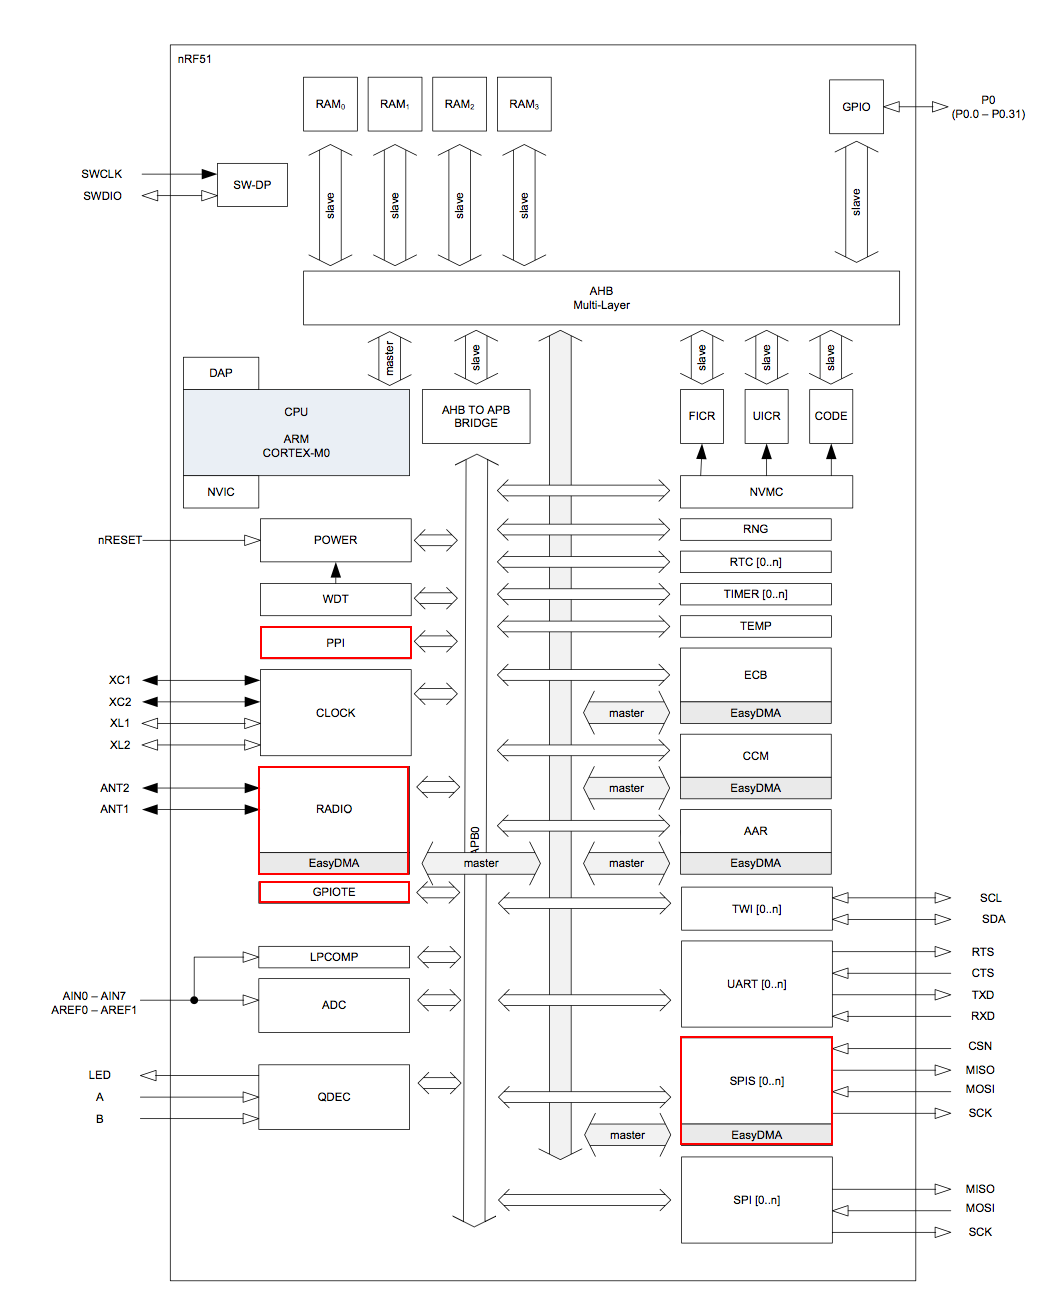
\includegraphics[scale=0.5]{fig/nrf51822_edit2.png}
\caption{Nordic nRF51 System architecture \cite{nrf51}}
\label{fig:nrf51}
\end{figure}
\chapter{Possible IoT Applications for Ultra Low Power Accelerometers}

This chapter is about possible IoT applications for low power accelerometers.

\section{Types of measurement}

Consumer grade MEMS accelerometers can typically measure from a range of $\pm2g$ to a range of $\pm16g$. This range is perfectly suited for measuring motion and vibration.  However, this range excludes shock and impact detection, as these events typically range in units of several hundred or even thousands of g's.

Light vibrations are in the order of 0.014 - 0.039g's, while the highest recorded earthquake was at its peak 2.99g's. The Bugatti Veyron supercar pulls 1.55g's when doing 0-100km/h in 2.4 seconds, while the space shuttle pulls at most 3g's during launch and reentry. A F-16 fighter jet is at most able to pull 9g-12g for limited amount of time.  while a baseball struck by a baseball bat is in the order of 3000g's.

For most accelerometer IoT applications it is therefore more than sufficient to be able to sense in range of $\pm2g$'s. There are however corner-cases. If the accelerometer for instance is to be used inside a baseball bat or soccer ball one might consider an accelerometer which a much higher measurement range.


\subsection{Vibration Detection}

For some construction applications it can be very beneficial to be able to monitor the vibrations inside the structure itself. Ultra low power sensors can for instance be submersed inside concrete walls and transmit during the entire life-span of the building. From this application one can really see the problem with changing batteries. As one would literally need to tear down a wall to change them. 

\subsection{Motion Detection}

In this thesis, a motion is regarded as slow moving event such as the movement of game controller or smart phone.

Motion detection can in it simplest form be used as a trigger to wake an external system. 
For some applications we might only be interested in the wake-up mode for an accelerometer. For such application it could be beneficial to use a special purpose device.

Motion Sensing is something that is being widely used in electronic devices today. It is for example being used as control input for certain smart phone applications.

\subsection{Health Monitoring}

Fitness armbands and smart watches is something that has gained much popularity in the recent years. These devices have quite strict requirements when it comes to size, so there is often not much room for a battery. For such applications it is therefore crucial to use ultra low power sensors and efficient data acquisition techniques. However, the sensors also need to have good enough performance to acquire useful data, such as the number of steps taken, heart rate information and so forth.  

\subsection{Pedometer}

...

\subsection{Navigation}

...
\chapter{Result}

This chapter presents the results from current measurement on the demo board application. 

\section{Power Analysis}

\subsection{Current Measurement}

A Keithly SMU has been used to measure current for the development...
%This is the Preface
%%=========================================
\chapter{Conclusion}

A study of MEMS based accelerometers has been carried out. The work has covered a wide range of topics with regards to the subject. Starting with the fundamental working principles of an accelerometer, continuing with different MEMS based implementations of an accelerometer. This has given useful information about some of the fundamental limitations, as well as some clear benefits with using the technology for future IoT applications. 

%mye å velge i, alle gode på sitt område, ut ifrra krieriene så har jeg valgt en...

This background theory has been the foundation for an analysis of five of the most low power accelerometers that are currently available on the market. The analysis has revealed that selecting a component for an embedded system is highly application specific, which makes it quite difficult to declare a winner that will be the obvious choice in every situation. The analysis has on the other hand showed that the ADXL362 from Analog Devices proves to be the most low power device currently available. This device also proves to be quite versatile, having a lot of different configuration options that can trade power for precision. This makes the accelerometer perfectly suited for a number of motion based IoT applications, whereas three  been proposed in this thesis. 

\section{Further Work}

A custom reference board using the ADXL362 from Analog Devices was designed as a part of this thesis. Several IoT applications has been proposed for this reference board in Chapter \ref{chap:applications}. For a future master thesis, the plan is to implement some of these applications using the reference board. 

%This is chapter 2
%%=========================================
\chapter[Equations]{Equations}
%The content of this chapter will vary with the topic of your thesis. 
%\begin{remark}
%If you want a shorter chapter or section title to appear in the Table of Contents and in the headings of the chapter, you just include the short title in square brackets before the title of the chapter/section.
%\end{remark}

%%=========================================
\section{Equations}
Relationship between power spectral density (PSD) and root-mean-square (RMS) \cite{freescale_accel_terminology}.

\begin{equation}
N^{2}_{rms}=\int_0^\infty{PSD(f)df}
\label{eq2}
\end{equation}

\begin{equation}
N^{2}_{rms}=\int_0^{BW}{PSD(f)df}
\label{eq3}
\end{equation}

\begin{equation}
N^{2}_{rms}=PSD \cdot (BW - 0)
\label{eq4}
\end{equation}

\begin{equation}
N_{rms}=\sqrt{PSD \cdot BW}
\label{eq5}
\end{equation}

\begin{equation}
PSD = \frac{N_{rms}}{\sqrt{BW}}
\label{eq6}
\end{equation}

Calculating the effective number of bits (ENOB), from \cite{freescale_accel_terminology}.

\begin{equation}
\frac{S_{rms}}{N_{rms}} = \frac{\frac{2^n}{2\sqrt{2}}}{\frac{1}{\sqrt{12}}} = 2^n \cdot \frac{\sqrt{3}}{\sqrt{2}}
\label{eq7}
\end{equation}

\begin{equation}
(\frac{S_{rms}}{N_{rms}})dB = 20\log{2^n \cdot \frac{\sqrt{3}}{\sqrt{2}}}
\label{eq8}
\end{equation}

\begin{equation}
(\frac{S_{rms}}{N_{rms}})dB = 20\log{2^n} + 20\log{1.225}
\label{eq9}
\end{equation}

\begin{equation}
(\frac{S_{rms}}{N_{rms}})dB = 602n + 1.76
\label{eq10}
\end{equation}

\begin{equation}
ENOB = \frac{SND(dB)-1.76}{6.02}
\end{equation}

% Include more chapters as required.
%%=========================================
\appendix
%This is Appendix A - Acronyms
%%=========================================

\chapter{Acronyms}
\begin{description}
\item[ODR] Output Data Rate
\item[MEMS] Microelectromechanical System
\item[IC] Integrated Circuit
\item[PPI] Peripheral Interconnect
\item[DMA] Direct Memory Access
\item[MCU] Microcontroller Unit
\item[SoC] System-on-Chip
\item[GPIOTE] General Purpose Input/Output Task Event
\item[ASIC] Application Specific Integrated Circuit
\item[BLE] Bluetooth Low Energy
\item[SPI] Serial Peripheral Interface
\item[I2C] Inter-Integrated Circuit
\item[CMOS] Complementary Metal-Oxide Semiconductor
\item[SRAM] Static Random-Access Memory
\item[ADC] Analog Digital Converter
\item[LSB] Least Significant Bit
\item[PSD] Power Spectral Density
\item[RMS] Root-Mean-Square
\item[BW] Bandwidth
\item[ENOB] Effective Number Of Bits
\item[SNR] Signal-to-Noise Ratio
\item[FIFO] First-In First-Out
\item[LIFO] Last-In First-Out
\item[PCB] Printed Circuit Board
\item[IoT] Internet of Things
\item[LED] Light Emitting Diode
\item[GPS] Global Positioning System
\end{description}
\chapter{PCB Schematic and 3D-Render}
\label{chap:appendix_a}

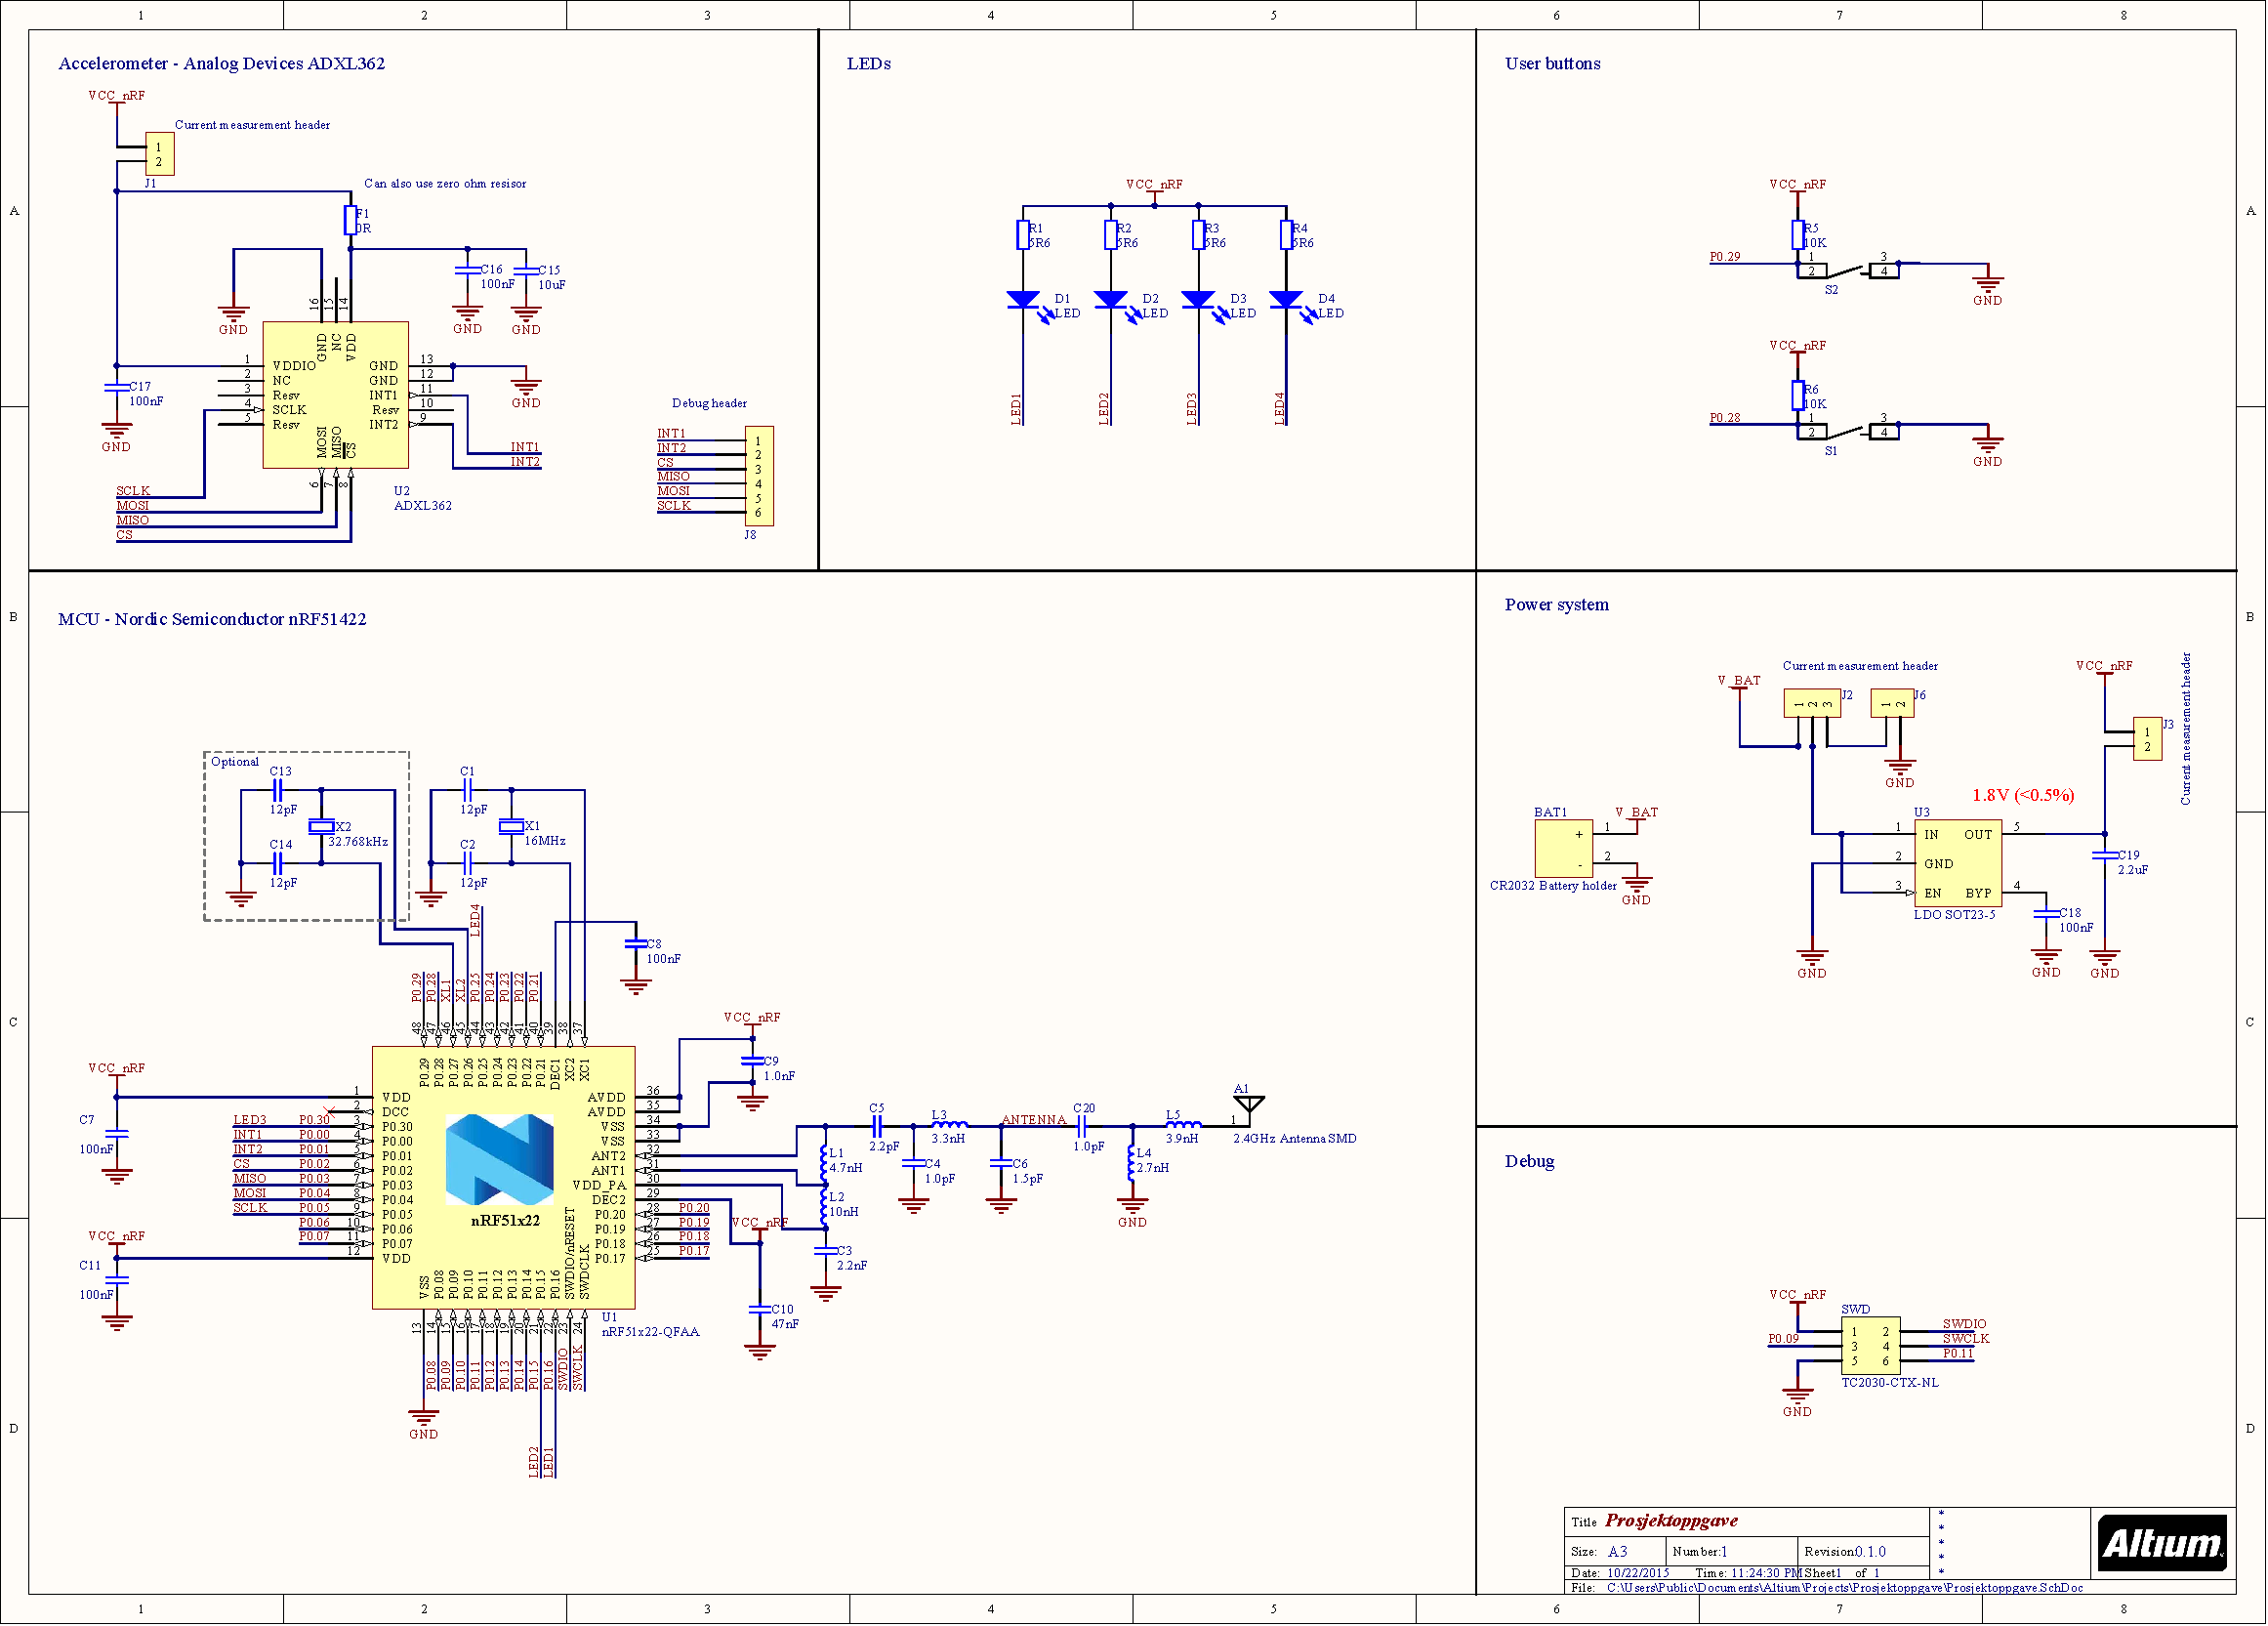
\includepdf[pages=-]{fig/schematic.PDF}
%This is an Appendix
%%=========================================

\chapter{Additional Information}
This is an example of an Appendix. You can write an Appendix in the same way as a chapter, with sections, subsections, and so on.

%%=========================================
\section{Introduction}

%%=========================================
\subsection{More Details}
% Include more appendices as required.
%%=========================================
\bibliographystyle{apa}
\addcontentsline{toc}{chapter}{\bibname}
\bibliography{refs}  
%%=========================================
\include{vitae}         % Your curriculum Vitae     
%%=============================================

\end{document}
